\documentclass{beamer}
\usepackage{risk231}   % shared preamble: packages, theorems, colours, listings

\setchapter{3}         % sections numbered 3.1, 3.2, ...

\title{RISK 231: VBA}

% local helpers for this chapter
\tikzset{
  note/.style={draw=black!70, fill=white, align=left, font=\scriptsize, inner sep=3pt},
  rednote/.style={draw=red!70!black, thick, fill=white, align=left, font=\scriptsize, inner sep=3pt},
  ptr/.style={-{Latex}, thin, black!70},
  rptr/.style={-{Latex}, red!70!black, thick}}
% code-like template text with italic placeholders, e.g. \tpl{Dim} \ph{Variable Name}
\newcommand{\kw}[1]{\textbf{\texttt{\color{blue!70!black}#1}}}
\newcommand{\ph}[1]{\textit{\texttt{\{#1\}}}}

\begin{document}
\maketitle

%======================================================================
\section{VBA: Intro, the VBE, and Recording Macros}
%======================================================================

\sectionframe

\begin{frame}{What is VBA?}
\begin{itemize}
  \item ``Visual Basic for Applications''
  \item A programming language built into Excel
  \begin{itemize}
    \item Make sophisticated workbooks
    \item Write custom functions
  \end{itemize}
  \item What is a \textbf{macro}?
  \begin{itemize}
    \item A collection of code that performs a series of commands
    \item Very useful when doing repetitive jobs to improve efficiency
    \item In Excel, macros can be written or recorded
  \end{itemize}
  \item This website has a long list of things you can do with VBA, and tutorials:
  \begin{center}
    \url{http://www.excel-easy.com/vba.html}
  \end{center}
\end{itemize}
\end{frame}

\begin{frame}{Why use VBA?}
\begin{itemize}
  \item \textbf{Automate a manual and repetitive process to save time and
        eliminate human error}
\end{itemize}
\end{frame}

\begin{frame}{The Visual Basic Editor (VBE)}
\begin{columns}[T]
\begin{column}{0.24\textwidth}
\small
Open the VBE from the \textbf{Developer} tab: click \textbf{Visual Basic}.

\vspace{0.5em}
\includegraphics[width=\linewidth]{ch03/developer_visual_basic}
\end{column}
\begin{column}{0.75\textwidth}
\centering
\includegraphics[width=\linewidth]{ch03/vbe_window}
\end{column}
\end{columns}
\end{frame}

\begin{frame}[fragile]{The Visual Basic Editor: getting code into a module}
\begin{itemize}
  \item Before you can do anything meaningful, you must have some VBA code in the
        VBA module. You can get VBA code into a VBA module in three ways:
  \begin{itemize}
    \item \textbf{Use the Excel macro recorder to record your actions and convert them to VBA code.}
    \item \textbf{Enter the code directly.}
    \item \textbf{Copy the code from one module and paste it into another.}
  \end{itemize}
\end{itemize}
\red{Entering the code directly:}

\begin{columns}[T]
\begin{column}{0.42\textwidth}
\includegraphics[width=\linewidth]{ch03/developer_macros}

\small\red{Name your macro (e.g.\ NewMacro) and click ``Create''.}
\end{column}
\begin{column}{0.55\textwidth}
\begin{lstlisting}[language=VBA]
Sub NewMacro()

    MsgBox "Hello World"

End Sub
\end{lstlisting}
\small Run it with the \textbf{Run} button
(\textcolor{dgreen}{$\blacktriangleright$}) on the VBE toolbar (or press F5).
\end{column}
\end{columns}
\end{frame}

\begin{frame}{The Visual Basic Editor: buttons and other cool things\ldots}
\begin{columns}[c]
\begin{column}{0.45\textwidth}
\includegraphics[width=\linewidth]{ch03/developer_insert_button}
\end{column}
\begin{column}{0.5\textwidth}
\begin{itemize}
  \item \textbf{Developer} $\to$ \textbf{Insert} $\to$ \textbf{Form Controls}
        $\to$ \textbf{Button (Form Control)}.
  \item Put the button wherever you want and assign it to your new macro.
\end{itemize}
\end{column}
\end{columns}
\end{frame}

\begin{frame}{Recording a Macro}
\red{Using the Excel macro recorder to record your actions and convert them to VBA code:}

\vspace{0.6em}
\begin{center}
\begin{tikzpicture}
  \node[inner sep=0] (rib) {\includegraphics[width=0.42\textwidth]{ch03/developer_record_macro}};
  \node[right=0.6cm of rib] (or) {or};
  \node[right=0.6cm of or, inner sep=0] {\includegraphics[width=0.22\textwidth]{ch03/statusbar_record_macro}};
\end{tikzpicture}
\end{center}
\vspace{0.6em}
\begin{itemize}
  \item Name your new macro, put in a shortcut key (if you'd like). Do stuff, then push stop.
  \item You can then see the automatically written code and adjust as desired.
\end{itemize}
\end{frame}

\begin{frame}{Some coding rules and good habits}
\begin{itemize}
  \item White space is ignored in VBA and the editor will automatically discard any extra spaces.
  \begin{itemize}
    \item Always put a space after a comma, never before, just like in regular English.
    \item Most infix operators (\code{=}, \code{+}, \code{-}, etc.) should always be surrounded by spaces.
    \item There are a few exceptions, which should never be surrounded by spaces,
          for example: power (\code{\^{}}), \code{\$}, \code{@}.
  \end{itemize}
  \vspace{0.4em}
  \item Indentation should be used to highlight the block structure and control statements.
  \begin{itemize}
    \item You can use the ``\textbf{Tab}'' key to indent your lines of code that logically
          belong together to make the code easier to read.
    \item The ``\textbf{Tab}'' key should be used instead of pressing the spacebar multiple times.
  \end{itemize}
\end{itemize}
\end{frame}

%======================================================================
\section{VBA: Variables and Objects}
%======================================================================

\sectionframe

\begin{frame}{Common Variable Types}
\centering\footnotesize
\begin{tabular}{@{}l >{\raggedright\arraybackslash}p{0.44\textwidth} >{\raggedright\arraybackslash}p{0.32\textwidth}@{}}
\toprule
\textbf{Type} & \textbf{Description} & \textbf{Examples}\\
\midrule
\code{Integer} & Any whole numbers from $-32{,}768$ to $32{,}767$ & 0, $-1$, 3, $-12{,}345$, 80\\[2pt]
\code{Long}    & Same as Integers, but can accept a much wider range (plus or minus 2 billion) & 1,849,418, $-766{,}484$\\[2pt]
\code{Double}  & Double-precision floating point decimal & 3.14159, 0.01, 100.99, $-99{,}481{,}147.33544$\\[2pt]
\code{String}  & Contains an array of characters & ``String Example1'', ``SFU''\\[2pt]
\code{Boolean} & True or false variable used for logic statements & TRUE, FALSE\\[2pt]
\code{Variant} & Variable that can take any of the above forms (and more). Requires larger amounts of system memory & All of the above\\
\bottomrule
\end{tabular}
\end{frame}

\begin{frame}{Declaring Variables}
Before a variable is used, it must be declared by using the \kw{Dim} statement.

\vspace{0.3em}
\centering
\begin{tikzpicture}
  \node (stmt) at (5.2,0) {\kw{Dim} \ph{Variable Name} \kw{As} \ph{Variable Type}};
  \node[note, text width=5.0cm, anchor=north west] (n1) at (0,-0.7) {%
    You can name a variable anything you want, subject to a few rules:
    \begin{itemize}\setlength{\itemsep}{0pt}
      \item Must begin with a letter
      \item Cannot contain spaces (use an underscore instead)
      \item Cannot be a ``reserved'' name (Ex: \code{Sub}, \code{Dim}, \code{If}, \code{True}, etc.)
      \item Cannot contain special characters (Ex: \code{+}, \code{-}, \code{\&}, \code{\$}, etc.)
    \end{itemize}};
  \node[note, text width=3.8cm, anchor=north west] (n2) at (6.0,-0.7) {%
    Variable type can be anything from the previous slide
    \begin{itemize}
      \item If you don't specify a variable type, the default is \code{Variant}
    \end{itemize}};
  \draw[ptr] ($(stmt.south west)!0.32!(stmt.south east)$) -- (n1.north);
  \draw[ptr] ($(stmt.south west)!0.82!(stmt.south east)$) -- (n2.north);
\end{tikzpicture}

\raggedright\small
\begin{itemize}
  \item Multiple variables can be declared in a single \kw{Dim} statement via comma separation.
  \item If you use a variable without declaration, it will be assumed as \code{Variant} (NOT recommended).
\end{itemize}
\end{frame}

\begin{frame}[fragile]{Assign values to variables}
To store data into a variable is called \emph{assignment}.

\vspace{0.3em}
\centering
\begin{tikzpicture}
  \node (stmt) at (5.2,0) {\kw{[Let]} \ph{Variable Name} \kw{=} \ph{Data}};
  \node[note, text width=4.2cm, anchor=north west] (n1) at (1.0,-0.7) {%
    Here ``Let'' usually can be ignored (i.e.\ we usually just write
    \ph{Variable Name} \texttt{=} \ph{Data}).};
  \node[note, text width=3.4cm, anchor=north west] (n2) at (6.4,-0.7) {%
    Assign data value on the right to the variable on the left.};
  \draw[ptr] ($(stmt.south west)!0.08!(stmt.south east)$) -- (n1.north);
  \draw[ptr] ($(stmt.south west)!0.72!(stmt.south east)$) -- (n2.north);
\end{tikzpicture}

\raggedright
\textbf{Example:}
\begin{columns}[c]
\begin{column}{0.5\textwidth}
\begin{lstlisting}[language=VBA]
Dim MyVariable As Integer
MyVariable = 2
\end{lstlisting}
\end{column}
\begin{column}{0.42\textwidth}
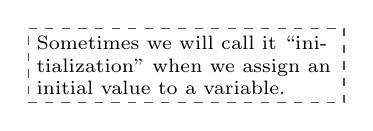
\begin{tikzpicture}
\node[note, dashed, text width=3.8cm] {Sometimes we will call it ``initialization''
  when we assign an initial value to a variable.};
\end{tikzpicture}
\end{column}
\end{columns}
\end{frame}

\begin{frame}[fragile]{Try it: declaration and \texttt{TypeName}}
\begin{columns}[T]
\begin{column}{0.45\textwidth}
\begin{lstlisting}[language=VBA]
Sub Test()

    Dim x, y As Integer
    z = 1
    MsgBox TypeName(x)

End Sub
\end{lstlisting}
\end{column}
\begin{column}{0.52\textwidth}
\small
\begin{itemize}
  \item \code{TypeName(x)} returns the type of \code{x} as a string.
  \item In \code{Dim x, y As Integer} only \code{y} is an \code{Integer};
        \code{x} has no type of its own, so it is a \code{Variant}.
  \item \code{z} is never declared, so it is also a \code{Variant}.
\end{itemize}
\end{column}
\end{columns}
\end{frame}

\begin{frame}[fragile]{Why do variable types matter?}
Run these three procedures and compare the message boxes:
\begin{columns}[T]
\begin{column}{0.32\textwidth}
\begin{lstlisting}[language=VBA]
Sub VtypeDemo1()
    Dim x as Integer
    x = 3.14
    MsgBox x
End Sub
\end{lstlisting}
\end{column}
\begin{column}{0.32\textwidth}
\begin{lstlisting}[language=VBA]
Sub VtypeDemo2()
    Dim x as Double
    x = 3.14
    MsgBox x
End Sub
\end{lstlisting}
\end{column}
\begin{column}{0.32\textwidth}
\begin{lstlisting}[language=VBA]
Sub VtypeDemo3()
    Dim x as Boolean
    x = 3.14
    MsgBox x
End Sub
\end{lstlisting}
\end{column}
\end{columns}
\end{frame}

\begin{frame}[fragile]{Examples with \texttt{Variant}}
To understand how \code{Variant} data types work, try executing these procedures:
\begin{columns}[T]
\begin{column}{0.48\textwidth}
\begin{lstlisting}[language=VBA]
Sub VariantDemo1()
    MyVar = "123"
    MyVar = MyVar + MyVar
    MyVar = "Answer: " & MyVar
    MsgBox MyVar
End Sub
\end{lstlisting}
\end{column}
\begin{column}{0.48\textwidth}
\begin{lstlisting}[language=VBA]
Sub VariantDemo2()
    MyVar = 123
    MyVar = MyVar + MyVar
    MyVar = "Answer: " & MyVar
    MsgBox MyVar
End Sub
\end{lstlisting}
\end{column}
\end{columns}
\end{frame}

\begin{frame}{Examples with \texttt{Variant} (cont.)}
\begin{itemize}
  \item For the first procedure, the message box displays \code{Answer: 123123}.
        As you assigned \code{MyVar} as \code{"123"}, it is implicitly considered as a text
        string, so the ``\code{+}'' operator will join (concatenate) the strings together.
  \vspace{0.6em}
  \item For the second procedure, the message box displays \code{Answer: 246}.
        As you assigned \code{MyVar} as \code{123}, it is implicitly considered as an integer,
        so the ``\code{+}'' operator will sum up the two values.
\end{itemize}
\end{frame}

\begin{frame}{Variable Scope}
A variable's \emph{scope} determines in which modules and procedures you can use the variable.

\vspace{0.6em}
\centering\small
\begin{tabular}{@{}>{\raggedright\arraybackslash}p{0.27\textwidth} >{\raggedright\arraybackslash}p{0.63\textwidth}@{}}
\toprule
\textbf{Scope} & \textbf{To Declare a Variable with This Scope}\\
\midrule
Single (Sub) procedure & Include a \code{Dim} or \code{Static} statement within the (Sub) procedure.\\[3pt]
Single module & Include a \code{Dim} or \code{Private} statement before the first procedure in a module.\\[3pt]
All modules & Include a \code{Public} statement before the first procedure in a module.\\
\bottomrule
\end{tabular}
\end{frame}

\begin{frame}{What are Objects?}
\begin{itemize}
  \item Objects are things that we can control or manipulate in Excel by VBA code.
  \item Structure of objects in Excel is like:
\end{itemize}
\centering
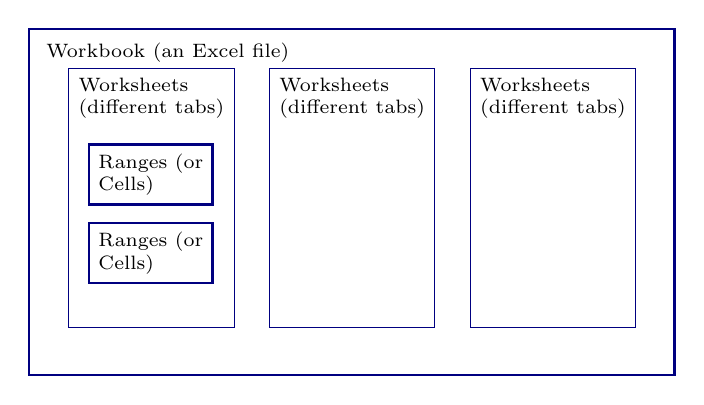
\begin{tikzpicture}[font=\scriptsize,
    wb/.style={draw=blue!50!black, thick},
    ws/.style={draw=blue!50!black, minimum width=2.1cm, minimum height=3.2cm, align=left, anchor=north west},
    rg/.style={draw=blue!50!black, thick, minimum width=1.5cm, minimum height=0.6cm, align=left}]
  \draw[wb] (0,0) rectangle (8.2,4.4);
  \node[anchor=north west, align=left] at (0.1,4.35) {Workbook (an Excel file)};
  \foreach \x in {0.5, 3.05, 5.6}
    \node[ws, text depth=2.6cm] at (\x,3.9) {Worksheets\\(different tabs)};
  \node[rg] at (1.55,2.55) {Ranges (or\\Cells)};
  \node[rg] at (1.55,1.55) {Ranges (or\\Cells)};
\end{tikzpicture}
\end{frame}

\begin{frame}{Common VBA Objects}
\centering\small
\begin{tabular}{@{}l >{\raggedright\arraybackslash}p{0.66\textwidth}@{}}
\toprule
\textbf{Objects} & \textbf{Descriptions}\\
\midrule
\code{Application} & Represents the Excel software application\\[2pt]
\code{Workbooks}   & Represents workbooks in Excel (an Excel file)\\[2pt]
\code{Worksheets}  & Represents worksheets in a workbook (it is just the tabs we usually refer to)\\[2pt]
\code{Sheets}      & Object that includes \code{Charts} and \code{Worksheets} objects. Sometimes
                     \code{Sheets} and \code{Worksheets} can be used interchangeably.\\[2pt]
\code{Range}       & Represents cells in an Excel worksheet; it can be a cell: \code{Range("A1")}
                     or a range: \code{Range("A1:B3")}\\[2pt]
\code{Cells}       & Represents a single cell in an Excel worksheet, specified by row number and
                     column number. For example: \code{Cells(3, 1)} is equivalent to \code{Range("A3")}.\\
\bottomrule
\end{tabular}
\end{frame}

\begin{frame}{Properties and Methods of Objects}
\textbf{Properties} are essentially the characteristics of an object.
\begin{center}
\begin{tikzpicture}
  \node (p) at (5,0) {\texttt{\large Range("A1").Value}};
  \node[note, anchor=north] (o) at (1.2,-0.75) {\textbf{Object}: Cell A1};
  \node[note, text width=2.6cm, anchor=north] (d) at (4.6,-0.75) {Object and property are connected with dot};
  \node[note, text width=2.4cm, anchor=north] (v) at (8.3,-0.75) {\textbf{Value}: refers to the value in this cell};
  \draw[ptr] ($(p.south west)!0.25!(p.south east)$) -- (o.north);
  \draw[ptr] ($(p.south west)!0.57!(p.south east)$) -- (d.north);
  \draw[ptr] ($(p.south west)!0.8!(p.south east)$) -- (v.north);
\end{tikzpicture}
\end{center}
\vspace{-0.3em}
{\small There are some other properties like \code{Name}, \code{Rows.Count}.}

\vspace{0.6em}
\textbf{Methods} are the actions that can be performed with an object.
\begin{center}
\begin{tikzpicture}
  \node (m) at (5,0) {\texttt{\large Range("A1").Select}};
  \node[note, text width=3.6cm, anchor=north] (s) at (7.6,-0.7) {\textbf{Select}: action to the cell, means select this cell};
  \draw[ptr] ($(m.south west)!0.85!(m.south east)$) -- (s.north);
\end{tikzpicture}
\end{center}
\vspace{-0.3em}
{\small There are also some other usual methods like \code{Copy}, \code{Paste}, \code{ClearContents}, etc.}
\end{frame}

\begin{frame}[fragile]{Understanding Objects}
\begin{itemize}
  \item To point to a specific object in VBA, you can traverse the object model.
        For example, to get to cell A1 on Sheet 1, you can enter this code:
\begin{lstlisting}[language=VBA]
Application.ThisWorkbook.Sheets("Sheet1").Range("A1").Select
\end{lstlisting}
  \item Entering this code also gets you to cell A1 because Excel infers that you mean
        the current workbook and the active sheet:
\begin{lstlisting}[language=VBA]
Range("A1").Select
\end{lstlisting}
  \item Indeed, if you have your cursor already in cell A1, you can simply use the
        \code{ActiveCell} object, negating the need to spell out the range.
\begin{lstlisting}[language=VBA]
ActiveCell.Select
\end{lstlisting}
\end{itemize}
\end{frame}

\begin{frame}{Some Other Useful Objects}
\centering
\begin{tabular}{@{}l >{\raggedright\arraybackslash}p{0.6\textwidth}@{}}
\toprule
\textbf{Objects} & \textbf{Descriptions}\\
\midrule
\code{ActiveCell}     & The active cell.\\[2pt]
\code{ActiveSheet}    & The active sheet.\\[2pt]
\code{ActiveWorkbook} & The active workbook.\\[2pt]
\code{Selection}      & The object selected. It could be a \code{Range} object, \code{Chart} object and so on.\\
\bottomrule
\end{tabular}
\end{frame}

\begin{frame}[fragile]{Assign Values to Object Variables}
We can also declare a variable of an object type and assign object data to it:

\vspace{0.4em}
\centering
\begin{tikzpicture}
  \node[anchor=west] (d) at (0,0) {\kw{Dim} \ph{Object Variable Name} \kw{As} \ph{Object Type}};
  \node[note, anchor=north east] (t) at ($(d.south east)+(0.3,-0.35)$) {Can be: \code{Range}, \code{Worksheet}, \code{Workbook}};
  \draw[ptr] ($(d.south east)+(-0.9,0.05)$) -- ($(t.north east)+(-0.6,0)$);
  \node[anchor=west] (s) at (0,-1.5) {\kw{Set} \ph{Object Variable Name} \kw{=} \ph{Object Data}};
  \node[note, anchor=north west] (m) at ($(s.south west)+(0,-0.35)$) {\textbf{MUST} have ``Set'' here};
  \draw[ptr] ($(s.south west)+(0.35,0.05)$) -- ($(m.north west)+(0.35,0)$);
\end{tikzpicture}

\raggedright
\textbf{Example:}
\begin{lstlisting}[language=VBA]
Dim rng As Range
Set rng = Range("A1:B8")
\end{lstlisting}
\end{frame}

\begin{frame}{\texttt{InputBox}}
One can directly receive an input value from the user and use it as a variable in VBA
via \textbf{InputBox}.

\vspace{0.4em}
\begin{center}\small
\ph{Variable Name} \texttt{=}\\[2pt]
\quad\kw{Application.InputBox}\texttt{(prompt:="[your message]", Type:=??)}
\end{center}

\centering\small
\begin{tabular}{@{}c l@{}}
\toprule
\textbf{Value for \code{Type}} & \textbf{Description}\\
\midrule
0  & A formula\\
1  & A number\\
2  & Text (a string)\\
4  & A logical value (\textbf{True} or \textbf{False})\\
8  & A cell reference, as a \textbf{Range} object\\
16 & An error value, such as \code{\#N/A}\\
64 & An array of values\\
\bottomrule
\end{tabular}
\end{frame}

\begin{frame}[fragile]{\texttt{MsgBox}}
One can display the value of a variable (along with pre-specified strings).
\begin{columns}[T]
\begin{column}{0.48\textwidth}
\begin{lstlisting}[language=VBA]
Sub MsgBoxDemo1()
    MyVar = 123
    MsgBox MyVar
End Sub
\end{lstlisting}
\begin{lstlisting}[language=VBA]
Sub MsgBoxDemo2()
    MyVar = 123
    MsgBox "My value is " & MyVar
End Sub
\end{lstlisting}
\end{column}
\begin{column}{0.48\textwidth}
\begin{lstlisting}[language=VBA]
Sub MsgBoxDemo3()
    x = 2
    y = 4
    z = x + y
    MsgBox x & " + " & y & " = " & z
End Sub
\end{lstlisting}
\end{column}
\end{columns}
\end{frame}

%======================================================================
\section{VBA: If Statements, Loops, and Functions}
%======================================================================

\sectionframe

\begin{frame}{If Statements -- Excel}
\begin{itemize}
  \item An \textbf{IF} statement is the most commonly used control statement.
  \vspace{0.5em}
  \item We've learned the Excel version:
  \begin{center}\small
    \code{=IF( \{condition\}, \{value if true\}, \{value if false\} )}
  \end{center}
  \begin{itemize}
    \item \{Condition\} is an expression that evaluates to a Boolean (true / false) data type.
    \item If the expression returns true, the \{value if true\} expression is returned.
          If false, the \{value if false\} expression is returned.
  \end{itemize}
  \vspace{0.5em}
  \item The VBA version works almost the same way. There's just different notation
        and a little more flexibility.
\end{itemize}
\end{frame}

\begin{frame}[fragile]{If \ldots\ Then Statements}
\begin{itemize}
  \item Below is an example of a simple \kw{If} \ldots\ \kw{Then} statement in VBA.
\begin{lstlisting}[language=VBA]
If {Condition} Then
    {Stuff}
End If
\end{lstlisting}
  \item Read the statement like this:
  \begin{itemize}
    \item \textbf{If} the condition is true, \textbf{Then} execute the commands between
          \texttt{Then} and \textbf{End If}. If the condition is false, then go to the line after
          \texttt{End If}.
  \end{itemize}
  \item The condition piece often features logical arguments (\code{True}, \code{False}, \code{<}, \code{>}, etc.)
  \item Inside a condition, ``\code{=}'' is a test of equivalence. It is \underline{not} an assignment statement.
\end{itemize}
\end{frame}

\begin{frame}[fragile]{If \ldots\ Then \ldots\ Else Statements}
\begin{itemize}
  \item This expanded statement is analogous to the IF function in Excel.
  \item Read the statement like this:
  \begin{itemize}
    \item \textbf{If} the condition is true, \textbf{Then} execute the commands between
          \texttt{Then} and \textbf{Else}. If the condition is false, then execute the commands
          between \textbf{Else} and \textbf{End If}.
  \end{itemize}
\end{itemize}
\begin{center}
\begin{minipage}{0.5\textwidth}
\begin{lstlisting}[language=VBA]
If {Condition} Then
    {Stuff}
Else
    {Different Stuff}
End If
\end{lstlisting}
\end{minipage}
\end{center}
\end{frame}

\begin{frame}[fragile]{If \ldots\ Then \ldots\ ElseIf Statements}
\begin{itemize}
  \item Read the statement like this:
  \begin{itemize}
    \item \textbf{If} the condition is true, \textbf{Then} execute the commands between
          \texttt{Then} and \textbf{ElseIf}. If the condition is false, then \ldots
    \item If the \underline{second} condition is true, \textbf{Then} execute the commands
          between the \underline{second} \texttt{Then} and \textbf{End If}.
  \end{itemize}
\end{itemize}
\begin{center}
\begin{minipage}{0.6\textwidth}
\begin{lstlisting}[language=VBA]
If {Condition} Then
    {Stuff}
ElseIf {Different Condition} Then
    {Different Stuff}
End If
\end{lstlisting}
\end{minipage}
\end{center}
\end{frame}

\begin{frame}[fragile]{If \ldots\ Then \ldots\ ElseIf \ldots\ ElseIf \ldots\ Else Statements}
\begin{columns}[T]
\begin{column}{0.45\textwidth}
\begin{itemize}
  \item You can create very complex and robust if statements by combining the concepts
        on the past few slides.
\end{itemize}
\end{column}
\begin{column}{0.5\textwidth}
\begin{lstlisting}[language=VBA]
If {Condition} Then
    {Stuff}
ElseIf {Condition 2} Then
    {Stuff 2}
ElseIf {Condition 3} Then
    {Stuff 3}
ElseIf {Condition 4} Then
    {Stuff 4}
ElseIf {Condition 5} Then
    {Stuff 5}
ElseIf {Condition 6} Then
    {Stuff 6}
Else
    {Stuff 7}
End If
\end{lstlisting}
\end{column}
\end{columns}
\end{frame}

\begin{frame}[fragile]{Nesting}
\vspace{-0.4em}
\begin{itemize}
  \item A control structure is said to be \underline{nested} if it lives inside a control
        structure of a similar type.
  \item These equivalent examples highlight a nested if statement in both Excel and VBA.
  \item The \blue{highlighted} statements are nested because they are located entirely within
        the confines of an existing if statement.
\end{itemize}
\begin{columns}[T]
\begin{column}{0.45\textwidth}
\textbf{Excel Formula}

\footnotesize\code{=IF(A1<>0,}\\
\hspace*{1.5em}\code{\blue{IF(A1>0,LN(A1),LN(-A1))},}\\
\hspace*{1.5em}\code{0)}

\vspace{0.6em}
``\code{<>}'' means \emph{not equal to}.
\end{column}
\begin{column}{0.5\textwidth}
\textbf{VBA Statements}
\begin{lstlisting}[language=VBA,escapechar=!]
Function X(ByVal Y As Double) _
    As Double

    If Y <> 0 Then
!\color{blue}\ttfamily\ \ \ \ \ \ \ \ If Y > 0 Then!
!\color{blue}\ttfamily\ \ \ \ \ \ \ \ \ \ \ \ X = Log(Y)!
!\color{blue}\ttfamily\ \ \ \ \ \ \ \ Else!
!\color{blue}\ttfamily\ \ \ \ \ \ \ \ \ \ \ \ X = Log(-Y)!
!\color{blue}\ttfamily\ \ \ \ \ \ \ \ End If!
    Else
        X = 0
    End If
End Function
\end{lstlisting}
\end{column}
\end{columns}
\end{frame}

\begin{frame}[fragile]{Two Observations When Using Functions}
\vspace{-0.3em}
\textbf{1. Using parentheses to enclose arguments while using functions:}
\begin{itemize}
  \item \textbf{A simple rule}: if a function call is the ONLY statement on the line,
        parentheses aren't needed.
\begin{lstlisting}[language=VBA]
Sub MsgBoxDemo4()
    MsgBox "Hello World"
End Sub
\end{lstlisting}
  \item Otherwise (if there are other statements or elements), parentheses MUST be added
        to distinguish function arguments and other statements.
\begin{lstlisting}[language=VBA]
Sub MsgBoxDemo5()
    Dim ans As Integer
    ans = MsgBox("Continue?", vbYesNo)
End Sub
\end{lstlisting}
  \item See also:
  \href{https://www.automateexcel.com/vba/message-box/}{Creating Custom Message Boxes
  with VBA MsgBox Function (automateexcel.com)}
\end{itemize}
\end{frame}

\begin{frame}[fragile]{Two Observations When Using Functions (cont.)}
\textbf{2. When you use a function, you can either}
\begin{itemize}
  \item supply arguments \emph{positionally}, in the order that they appear in the
        procedure's definition:
\end{itemize}
\begin{lstlisting}[language=VBA]
Sub MsgBoxDemo6()
    MsgBox "Choose Yes or No", vbYesNo, "Selection Window"
End Sub
\end{lstlisting}
\begin{center}\scriptsize
\begin{tabular}{@{}ccc@{}}
\code{"Choose Yes or No"} & \code{vbYesNo} & \code{"Selection Window"}\\
$\downarrow$ & $\downarrow$ & $\downarrow$\\
\fcolorbox{red!70!black}{white}{Prompt} & \fcolorbox{red!70!black}{white}{Buttons} & \fcolorbox{red!70!black}{white}{Title}
\end{tabular}
\end{center}
\begin{itemize}
  \item or you can supply the arguments \emph{by name} without regard to position:
\begin{lstlisting}[language=VBA]
Sub MsgBoxDemo7()
    MsgBox prompt:="Hello World", Title:="This is a title"
End Sub
\end{lstlisting}
  \item A \textbf{named argument} consists of an argument name followed by a colon and an
        equal sign (\code{:=}), followed by the argument value.
\end{itemize}
\end{frame}

\begin{frame}[fragile]{InputBox Function Example}
\begin{lstlisting}[language=VBA]
Sub GetValue()
    Dim Monthly As Integer
    Monthly = Application.InputBox("Enter your monthly salary:", _
        Title:="Annual Salary Calculator", Type:=1)
    MsgBox "Annualized: $" & (Monthly * 12)
End Sub
\end{lstlisting}
\begin{itemize}
  \item \code{Type:=1} restricts your input to be numbers.
  \item The underscore \code{\_} at the end of a line continues the statement on the next line.
  \item The input box shows up when the code is executed:
\end{itemize}
\begin{center}
\includegraphics[width=0.5\textwidth]{ch03/inputbox_salary_dialog}
\end{center}
\end{frame}

\begin{frame}{For-Next Loops}
\begin{itemize}
  \item \textbf{For-Next Loops} are an easy, extremely useful way to repeat structurally
        similar tasks many times over.
  \item Mathematical notation: \quad $\displaystyle\sum_{i=1}^{n} X_i$ \qquad $\displaystyle\prod_{i=1}^{n} X_i$
\end{itemize}
\centering
\begin{tikzpicture}[font=\scriptsize]
  \node[draw, thick, minimum width=5.2cm, minimum height=3cm] (box) at (0,0) {};
  \node[draw, anchor=south] (for) at ($(box.north west)+(-0.3,0.5)$) {\texttt{For i = 1 to n}};
  \draw (for.south west) -- (box.north west);
  \draw (for.south east) -- (box.north east);
  \node at ($(box.center)+(-1.45,0)$) {Body of Loop};
  \node at ($(box.center)+(1.75,0.25)$) {\texttt{Next i}};
  \draw[line width=4pt, -{Latex[length=7pt]}, cyan!40] ($(box.center)+(-0.9,0.5)$)
       to[bend left=40] ($(box.center)+(0.9,0.6)$);
  \draw[line width=4pt, -{Latex[length=7pt]}, cyan!40] ($(box.center)+(0.9,-0.5)$)
       to[bend left=40] ($(box.center)+(-0.9,-0.6)$);
  \node[starburst, draw, fill=white, inner sep=0pt, font=\scriptsize] (st) at ($(box.east)+(1.3,-0.4)$) {If i = n + 1};
  \node[draw, align=center, font=\tiny] (out) at ($(st)+(0,-1.7)$) {No more looping;\\continue with code};
  \draw[-{Latex}, thick, blue!60!black] (st.south) -- (out.north);
\end{tikzpicture}
\end{frame}

{% smaller list fonts for this dense slide
\setbeamerfont{itemize/enumerate body}{size=\scriptsize}
\setbeamerfont{itemize/enumerate subbody}{size=\scriptsize}
\begin{frame}[fragile]{For-Next Loop Format}
\begin{columns}[c]
\begin{column}{0.5\textwidth}
\begin{lstlisting}[language=VBA]
For {Index} = {low} To {high}
    {Body of Loop}
Next {Index}
\end{lstlisting}
\end{column}
\begin{column}{0.46\textwidth}
\small Read the statement like this: run the loop (high $-$ low $+ 1$) times, each time
increasing the value of the index by 1.
\end{column}
\end{columns}
\vspace{0.2em}
\scriptsize
Components of a For-Next Loop:
\begin{columns}[T]
\begin{column}{0.48\textwidth}
\begin{itemize}
  \item \blue{Index} -- execution of the loop hinges upon the value of an index variable
  \begin{itemize}
    \item The index should be an \code{Integer} or \code{Long} variable
    \item Don't forget to declare the index as a variable first!
  \end{itemize}
  \item \blue{Low Value} -- initial value an index takes
  \begin{itemize}\item On first loop iteration, Index = low value\end{itemize}
\end{itemize}
\end{column}
\begin{column}{0.48\textwidth}
\begin{itemize}
  \item \blue{High Value} -- final value an index takes
  \begin{itemize}\item On final loop iteration, Index = high value\end{itemize}
  \item \blue{Next} -- must be at the end of the loop
  \begin{itemize}
    \item If Index $<$ High Value, Index increases by 1 and the loop reruns (new iteration)
    \item If Index $=$ High Value, code continues to the statement below \code{Next}
  \end{itemize}
\end{itemize}
\end{column}
\end{columns}
\end{frame}
}

\begin{frame}[fragile]{Do Loops}
\begin{itemize}
  \item A \blue{Do Loop} is another common control structure used for repeating sections of code.
  \item Two types:
  \begin{itemize}
    \item Execute loop \blue{While} a certain condition exists
    \item Execute loop \blue{Until} a certain condition exists
  \end{itemize}
  \item Uses of a Do Loop
  \begin{itemize}
    \item Brute force solve methods
    \item Parameter calibration (e.g.)
    \begin{itemize}
      \item Refine estimate \emph{while} square error is greater than tolerance level
      \item Refine estimate \emph{until} square error is less than tolerance level
    \end{itemize}
  \end{itemize}
  \item Not as common as For Loops, but some notation is included in case you're interested.
\end{itemize}
\begin{columns}[T]
\begin{column}{0.4\textwidth}
\begin{lstlisting}[language=VBA]
Do While {Condition}
    {Stuff}
Loop
\end{lstlisting}
\end{column}
\begin{column}{0.4\textwidth}
\begin{lstlisting}[language=VBA]
Do Until {Condition}
    {Stuff}
Loop
\end{lstlisting}
\end{column}
\end{columns}
\end{frame}

\begin{frame}[fragile]{Some Looping Techniques}
\small
A usual application of loops is to populate values row by row. There are several ways to do it:
\begin{enumerate}
  \item Use the \code{Offset} method of the \code{Range} object.
  \item Use the \code{Cells} object.
  \item Use the \code{Range} object, incorporating a concatenation trick.
\end{enumerate}
\begin{columns}[T]
\begin{column}{0.64\textwidth}
\begin{lstlisting}[language=VBA,basicstyle=\ttfamily\fontsize{6.5}{8}\selectfont]
Sub LoopDemo()
    Dim i As Integer
    For i = 1 To 10
        ' Use Offset to populate col A
        Range("A1").Offset(i - 1, 0).Value = i
        ' Use Cells to populate col B
        Cells(i, 2).Value = i
        ' Use concatenate and Range to populate col C
        Range("C" & i).Value = i
    Next i
End Sub
\end{lstlisting}
\end{column}
\begin{column}{0.34\textwidth}
\centering
\includegraphics[height=2.4cm]{ch03/loopdemo_result}

\vspace{0.2em}
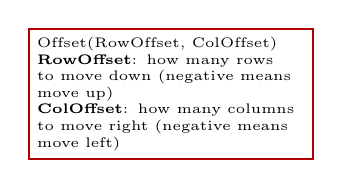
\begin{tikzpicture}
\node[rednote, text width=3.4cm, font=\tiny] {\code{Offset(RowOffset, ColOffset)}\\
  \textbf{RowOffset}: how many rows to move down (negative means move up)\\
  \textbf{ColOffset}: how many columns to move right (negative means move left)};
\end{tikzpicture}
\end{column}
\end{columns}
\end{frame}

\begin{frame}[fragile]{Some Looping Techniques: \texttt{Range.Count}}
\begin{itemize}
  \item \code{Range.Count} method:
  \begin{itemize}
    \item Returns a value that represents the number of objects (cells), no matter empty or nonempty.
    \item For example, the following statement returns value 8.
  \end{itemize}
\end{itemize}
\begin{center}
\begin{minipage}{0.45\textwidth}
\begin{lstlisting}[language=VBA]
MsgBox Range("A1:A8").Count
\end{lstlisting}
\end{minipage}
\end{center}
\begin{itemize}
  \item \red{\textbf{An important and useful technique}}: how to use VBA to determine how many
        records are in a table?
  \begin{itemize}
    \item This is a practical question because when you use a For-Next loop, you always want
          to know how many loops we should do (i.e.\ what is the High value?).
    \item In the following example, we are going to use a combination of methods:
          \code{Count} and \code{End}.
  \end{itemize}
\end{itemize}
\end{frame}

\begin{frame}[fragile]{Some Looping Techniques: \texttt{Range.End}}
\begin{itemize}
  \item \code{Range.End(\textit{Direction})} method:
  \begin{itemize}
    \item Returns a \code{Range} object that represents the cell at the end of the region
          that contains the source range.
    \item The argument \textit{Direction} could be: \code{xlDown}, \code{xlToRight},
          \code{xlToLeft} or \code{xlUp}.
    \item For example:
  \end{itemize}
\end{itemize}
\begin{tikzpicture}[keybox/.style={fill=blue!55!black, text=white, font=\small, inner sep=4pt}]
  \node[anchor=west, inner sep=0, text width=5.6cm] (c1) at (0,0) {%
\begin{lstlisting}[language=VBA]
Range("A1").End(xlToRight).Select
\end{lstlisting}};
  \node[keybox, below=0.15cm of c1] {Ctrl + $\rightarrow$};
  \node[single arrow, draw=red!70!black, fill=red, minimum height=0.8cm, right=0.3cm of c1] (a1) {};
  \node[inner sep=0, right=0.3cm of a1] {\includegraphics[width=3.4cm]{ch03/end_xltoright}};
  \node[anchor=west, inner sep=0, text width=5.6cm] (c2) at (0,-2.0) {%
\begin{lstlisting}[language=VBA]
Range("A1").End(xlDown).Select
\end{lstlisting}};
  \node[keybox, below=0.15cm of c2] {Ctrl + $\downarrow$};
  \node[single arrow, draw=red!70!black, fill=red, minimum height=0.8cm, right=0.3cm of c2] (a2) {};
  \node[inner sep=0, right=0.3cm of a2] {\includegraphics[width=3.4cm]{ch03/end_xldown}};
\end{tikzpicture}
\end{frame}

\begin{frame}[fragile]{Some Looping Techniques: \texttt{Count} and \texttt{End} together}
\small
\begin{itemize}
  \item Use a combination of \code{Count} and \code{End} to help us determine the number of
        records in a data table.
  \item Another expression using the \code{Range} object: \code{Range(\textit{Cell1}, [\textit{Cell2}])}
        can hold two objects. These are equivalent; both refer to the range from A1 to A5:
\end{itemize}
\begin{columns}[T]
\begin{column}{0.66\textwidth}
\begin{lstlisting}[language=VBA]
Range("A1:A5")
Range(Range("A1"), Range("A5"))
\end{lstlisting}
\begin{lstlisting}[language=VBA,basicstyle=\ttfamily\tiny]
Range(Range("B3"), Range("B3").End(xlDown)).Count
\end{lstlisting}
\scriptsize
\begin{itemize}
  \item \code{Range("B3")}: start from cell B3
  \item \code{Range("B3").End(xlDown)}: to the last cell in the column that contains cell B3;
        the range is what \colorbox{blue!55!black}{\textcolor{white}{Ctrl + Shift + $\downarrow$}} selects
  \item \code{.Count}: count the number of cells in this range
        $\Rightarrow$ 10 records (B3:B12)
\end{itemize}
\end{column}
\begin{column}{0.32\textwidth}
\centering
\includegraphics[width=\linewidth]{ch03/student_scores}
\end{column}
\end{columns}
\end{frame}

\end{document}
